\documentclass[]{standalone}

\usepackage{amsmath}
\usepackage{amsfonts}
\usepackage{amssymb}
\usepackage{graphicx}
\usepackage{tikz}
\usepackage{import}
\usepackage[subpreambles=true]{standalone}

\usepackage{tikz}
\usepackage{tikz-3dplot}

\usetikzlibrary{positioning}

\begin{document}

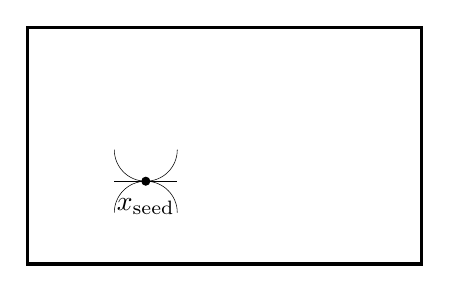
\begin{tikzpicture}[scale=1]
    % \path[draw, fill] (5.5, 3.0) circle (0.05) node[right]{$V_\mathrm{closed}$};
    % \path[draw, fill=gray] (5.5, 2.5) circle (0.05) node[right]{$V_\mathrm{open}$};
    % \path[draw, fill=white] (5.5, 2.0) circle (0.05) node[right]{$V_\mathrm{unvisited}$};

    \useasboundingbox (0,0) rectangle (5,3);

    \coordinate (init) at (0.5,0.5);
    \coordinate (goal) at (4.6,2.25);
    \coordinate (obs1) at (2.4,2.1);
    \coordinate (obs2) at (3.7,0.65);
    \coordinate (seed) at (1.5,1.05);
    
    \path[draw, fill=black] (seed) circle (0.05) node[below=1mm] {$x_\mathrm{seed}$};
    \path[draw, very thin] (seed) to ++(0.4,0);
    \path[draw, very thin] (seed) to[in=-90,out=0] ++(0.4,0.4);
    \path[draw, very thin] (seed) to[in=90,out=0] ++(0.4,-0.4);
    \path[draw, very thin] (seed) to ++(-0.4,0);
    \path[draw, very thin] (seed) to[in=-90,out=180] ++(-0.4,0.4);
    \path[draw, very thin] (seed) to[in=90,out=180] ++(-0.4,-0.4);
    

    % \path[draw=red, thick] (init) -- (n4) -- (n8) -- (n7) -- (n6) -- (goal);

    \path[draw, very thick] (0,0) -- (5,0) -- (5,3) -- (0,3) -- cycle;

    % \path[draw, fill=black] (init) circle (0.05) node[below] {$x_\mathrm{init}$};

    % \path[draw, fill=gray] (goal) circle (0.05) node[above] {$x_\mathrm{goal}$};

    % \path[draw, very thick, rounded corners=14pt, fill=black!30] (obs1) ++(-1.2,-1) -- ++(2,0.2) -- ++(0,1) -- ++(-1.5,0.5) -- cycle;
    % \path[draw, very thick, rounded corners=4pt, fill=black!30] (obs2) ++(-1.5,-0.25) -- ++(0,0.3) -- ++(1.3,0.2) -- ++(0.2,1) -- ++(0.3,0) -- ++(0.3,-1.6) -- cycle;

\end{tikzpicture}
\end{document}